%%--SubSkipper Documentation
%%--Modified 25/07/15

\documentclass{article}

%%--packages
\usepackage{hyperref}
\usepackage{color}
\usepackage{graphicx}
\graphicspath{{figures/}}
\usepackage{geometry}
\usepackage[table]{xcolor}
\usepackage{tabularx}

%%--Define Margins
 \geometry{
 a4paper,
 total={170mm,257mm},
 left=20mm,
 right=20mm,
 top=20mm,
 bottom=20mm,
 }


%%--commands
\newcommand{\degree}{$^{\circ}$}

\author{Filip Socko}
\title{Campaign Reference and Solution Aids}

\begin{document}

\maketitle
\pagebreak
\tableofcontents
\pagebreak

\section{Introduction}
The main purpose of this documentation is to record techniques and methods of early submarine attack techniques in a way which are simple to employ in computer programs (i.e. showing mathematical equations where possible), as well as acting as a reference for Submarine Simulators.
\\ \\
This document is a reference for Torpedo types and common conversion factors, as well as types of US Fleet Boats and Types of US Torpedoes. A brief recognition manual will be provided in an appendix. This document also aims to provide a brief overview of common torpedo solution methods.

\section{Unit Conversions}

\subsection{Length}
\begin{center}
\begin{tabular}{r | r}
$1.0$ NM & $1852.0$ m\\
$1.0$ NM & $2025.37$ yards\\
$1.0$ NM & $6076.12$ feet\\
$1.0$ km & $0.539956803$ NM\\
$1.0$ m & $3.2808399$ feet\\
$1.0$ m & $1.0936133$ yards\\
\end{tabular}
\end{center}

\subsection{Speed}

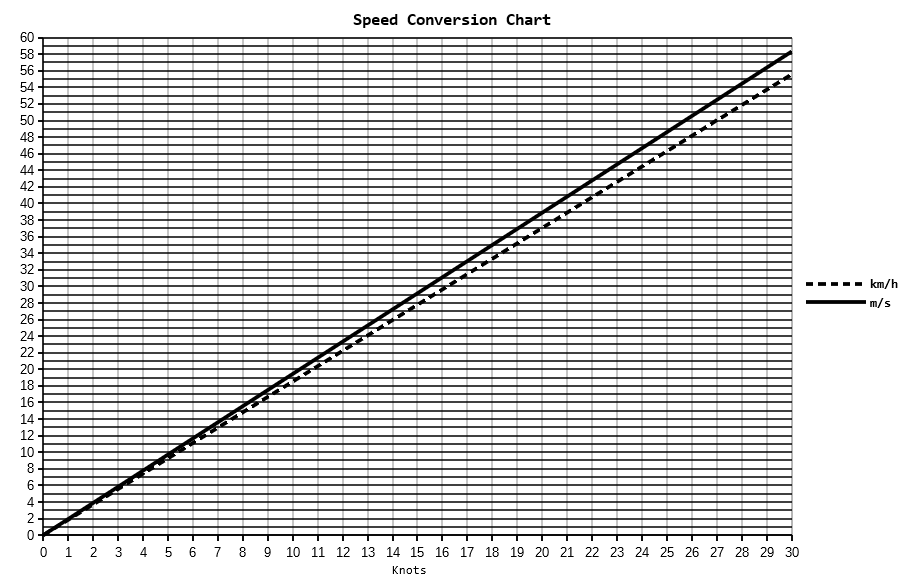
\includegraphics[width=\textwidth]{speedConversion}
\pagebreak

\section{Torpedo Data}

The following is torpedo for American torpedo types as used predominantly in the Pacific theatre.

Torpedo data adapted from \emph{SH4 V1.2 Ultimate Torpedo Guide} by Mechan, found at the ubisoft forums (http://forums.ubi.com/showthread.php/475595-SH4-V1-2-Ultimate-Torpedo-Guide-Forums). Dated: 06-22-2007, Accessed: 18.08.2015

Slow and Fast speeds and ranges removed as appropriate.

\subsubsection{Mark 10}
\begin{tabular}{l|l}
Available from:& Always\\
Range(m):& 3200\\
Speed(kt):&36\\
Warhead:& 80-160 radius 3-6m\\
Depth keeping:& 70\% chance of deviating $\pm 0.8m - \pm 1.2m$\\
Dud Chance (at AOB):& 1\% (0\degree -70\degree ) 25\% (70\degree-90\degree)\\
Renown cost:& 0\\
\end{tabular} \\
Notes: Default torpedo for the S-Class. Slower and with a shorter range than the Mk. 14, but extremely reliable.\\

\subsubsection{Mark 14}
\begin{tabular}{l|l}
Available from:& Always\\
Range(Slow)(m):& 8200\\
Range(Fast)(m):& 4100\\
Speed(Slow)(kt):&31\\
Speed(Fast)(kt):& 46\\
Warhead:& 100-170 radius 3-7m\\
Depth keeping:& 70\% chance of deviating $\pm 1.5m - \pm 3.3m$\\
Dud Chance (at AOB):& 1\% (0\degree-35\degree); 34\% (35\degree-70\degree); 99\% (70\degree-90\degree)\\
Renown cost:& 0\\
\end{tabular} \\
Notes: Default torpedo for all modern fleet boats. Faster and with a longer range than the Mk. 10, it packs a roughly 20\% stronger punch but is much less reliable.

\subsubsection{Mark 16}
\begin{tabular}{l|l}
Available from:& 1945-01-01\\
Range(m):& 12500\\
Speed(kt):&46\\
Warhead:& 180-250 radius 3.5-8m\\
Depth keeping:&  70\% chance of deviating $\pm 1.5m - \pm 3.3m$\\
Dud Chance (at AOB):& 4\% (0\degree-35\degree); 45\% (35\degree-70\degree); 100\% (70\degree-90\degree)\\
Renown cost:& 400\\
\end{tabular} \\
Notes: Fast torpedo with an exceptionally long range, but also terribly unreliable.

\subsubsection{Mark 18}
\begin{tabular}{l|l}
Available from:& 1943-07-12\\
Range(m):& 3650\\
Speed(kt):&29\\
Warhead:& 120-180 radius 3-7\\
Depth Keeping:& 55\% chance of deviating $\pm 1.2m - \pm 2.8m$\\
Dud Chance (at AOB):& 1\% (0\degree-35\degree); 34\% (35\degree-70\degree); 99\% (70\degree-90\degree)\\
Renown cost:&  500 (200 from 1944-01-16; 0 from 1944-09-01)\\
\end{tabular} \\
Notes: Slower, 10\% more powerful, with a shorter range and much more reliable than the Mk. 14.

\subsubsection{Mark 23}
\begin{tabular}{l|l}
Available from:& 1943-01-01\\
Range(m):& 4100\\
Speed(kt):&46\\
Warhead:& 120-180 radius 3-7m\\
Depth Keeping:& 70\% chance of deviating $\pm 1.5m - \pm 3.3m$\\
Dud Chance (at AOB):& 1\% (0\degree - 35\degree); 34\% (35\degree- 70\degree); 99\% (70\degree- 90\degree)\\
Renown cost:&  100 (0 from 16-01-1944)\\
\end{tabular} \\
Notes: Same range, speed and reliability than the Mk. 14 but roughly 10\% more powerful. Definitely replaces the Mk. 10 as the "standard" torpedo from 16-01-1944.

\subsubsection{Mark 27 "Cutie"}
\begin{tabular}{l|l}
Available From:& 1944-01-01\\
Range(m):& 4570\\
Speed(kt):&12\\
Warhead:& 50-100 radius 1.5-5\\
Depth Keeping:& NA\\
Dud Chance (at AOB):& 1\% (0\degree-25\degree)\\
Renown cost:& 500\\
\end{tabular} \\
Notes: Slow acoustic homing torpedo with a small warhead primarily used for defence against destroyers.

\subsubsection{Torpedo minimum arming distance}
\emph{arming\_distance} is set across all torpedoes to 220m except the Mk. 27, which is 150 meters.
\subsubsection{Torpedo max dive angle}
\emph{max\_dive\_angle} is set to 20 degrees for all torpedo types.
\subsubsection{Torpedo maximum turn angle}
\emph{max\_turn\_angle} is 135\degree for all torpedoes except the Mk. 27, which is 180\degree.
\subsubsection{Magnetic detonation range}
\emph{mag\_detonation\_range} is 2m for all torpedoes except for the Mk. 27, which is 1m.
\subsubsection{Circular runner torpedos}
\emph{circle\_runner\_chance} is 0.5\% for all torpedoes except for the Mk. 27, which is 0\%.
\subsubsection{Gyro problems}
The chance of having gyro problems is 0.3\% at the introduction time of all torpedoes and drops to 0.2\% in later periods for all torpedoes except for the Mk. 16. The \emph{max\_deviation} when having gyro problems is always 50\degree. This does not apply to the Mk. 27. 
\subsubsection{Homing torpedos}
The Mk. 27 will run straight for 200m before homing.

\section{Trigger Maru Overhaul - Fleet Boat Types}
This section consists of pages 25-28 of the Trigger Maru Overhaul Manual which detail fleet boat types:
\includegraphics[page={25}, width=\textwidth, height=.95\textheight]{TMO_Manual}
\includegraphics[page={26}, width=\textwidth, height=\textheight]{TMO_Manual}
\includegraphics[page={27}, width=\textwidth, height=\textheight]{TMO_Manual}
\includegraphics[page={28}, width=\textwidth, height=\textheight]{TMO_Manual}

%% Contents of original AngriffScheibe Handbuch which are relevant w/out the disk:
%Example 4: Determine the speed of a target by plotting position over time
%Example 5: Determine the speed of a target knowing the target length
%Example 6: Find the speed of a target with constant relative bearing
%EG. 7: Find the speed of a target with a changing relative bearing
%Example 8: Find the speed of a target with two bearing and range observations
%Example 9: Find the AOB of a target with the Aspect Ratio method
%Example 10: Determine the distance to the track of a target
%Example 11: Determine an optimum speed for attack position
%12: Determine the lead angle for a perpendicular attack with 0° gyro angle
%Example 13: Determine the torpedo gyro angle

%TODO

%Example 6: Find the speed of a target with constant relative bearing
%EG. 7: Find the speed of a target with a changing relative bearing
%Example 8: Find the speed of a target with two bearing and range observations
%Example 9: Find the AOB of a target with the Aspect Ratio method


\section{Calculating AOB Based on Aspect Ratio}

%Methods adapted from Angriffscheibe Handbuch by Karl Hahn, 2008.

AOB can be determined given the following data:
\begin{itemize}
\item{Observed Mast Height}
\item{Observed Ship Length}
\item{Reference Aspect Ratio (i.e. $\frac{Reference Length}{Reference Mast Height}$)}
\end{itemize}

\subsection{Determine an observed \emph{aspect ratio}.}
$$AR\_{observed} = \frac{Observed Length}{Observed Mast Height}$$
As the required figure is a ratio, it does not matter in what units the figures are given. For example, this could be the number of degrees Length and Mast Heigh subtend, the number of periscope graduations subtended or angular length in metres. It only matters that units for Observed Mast Height and Observed Length are the same.

\subsubsection{Determine the Reference Aspect Ratio}
Identify the target and find the Length and Mast Height as given in the recognition manual (if possible) or calculate these figures using the SubSkipper ship parser. Proceed as for the observed aspect ratio to get the Reference Aspect Ratio (\emph{ARreference}).

\subsection{AOB calculation}
$$AOB = arcSin \frac{AR\_{observed}}{AR\_{reference}}$$

\begin{itemize}
\item{Note: This method is less accurate as AOB approaches 0. Using this method with a sample size of 16 at various AOBs, the average error was 9.1\degree and the median error 6.88\degree. The optimum range for collecting data seems to be around 2000m.}
\item{Note: This method does not compute whether the AOB is on the port or starboard side.}
\item{Note: "The AOB can only go up to 90, and gives no indication of starboard or port side showing. You have to determine that visually.}

\item{
AOB (Relative to Target) for each Quadrant:
	\begin{itemize}
	\item{0\degree - 90\degree : Use AOB result as is.}
	\item{90\degree - 180\degree : Subtract AOB result from 180.}
	\item{180\degree - 270\degree : Subtract AOB result from 180.}
	\item{270\degree - 360\degree : Subtract AOB result from 360.}
	\end{itemize}

}
\end{itemize}

\section{Determine the distance to the track of a target}

As you manoeuvre into a firing position, it is useful to know your distance to the track of your target. Knowing the range and AOB of the target:

Track: intersection point between Submarine course and the current target course.

$$Distance to Track = Range \left( sin(AOB) \right)$$
%
%\section{Determine an optimum speed for attack position}
%
%To determine own speed needed to reach the target track in time to set up a torpedo solution. (Requires: Target Speed, Target AOB, Bearing to Target, Target Range, Distance to target track)
%
%\begin{enumerate}
%\item{Find distance T must travel to reach a bearing of 000\degree. If the track is known (see previous step) and bearing and range to target is known, time required is:
%$$ s = d/t  $$
%}


%Example 11: Determine an optimum speed for attack position


\section{Determine the lead angle for a perpendicular attack with 0\degree gyro angle (AKA O\'Kane Solution)}

Once you are turned onto a perpendicular intercept course, this method calculates when to fire. The lead angle is simply the target bearing at the moment you fire. The range is irrelevant to the calculation although it is best to plan the attack within 500-1000m.

$$ lead angle = tan^{-1} ( [target speed / torpedo speed] ) $$

\section{Determine the torpedo gyro angle}
This example will show how to calculate the required gyro angle for a firing solution. This method is somewhat simplified and is best for smaller gyro angles (\textless 30\degree) and shorter ranges (\textless 1000 metres).

$$sin (lead angle) / sin (AOB) = (target speed) / (torpedo speed)$$
$$ gyroAngle = targetBearing -– leadAngle $$

\section{O'Kane Table of Values}
\centering{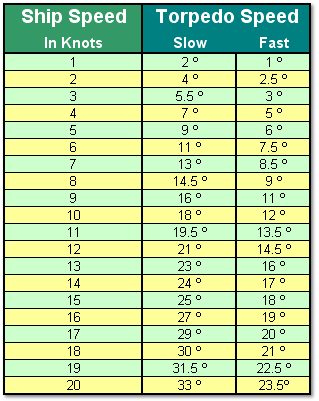
\includegraphics[height=10 cm]{OKaneValues}}

\pagebreak

\section{Torpedo spread at range (m) per angle of spread (\degree)}
\centering{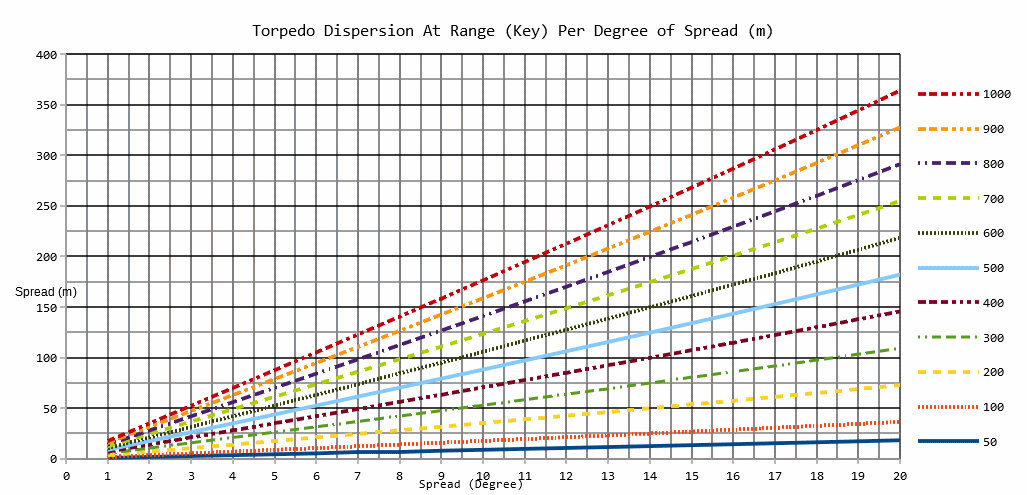
\includegraphics[width=\textwidth]{SpreadAtRange}}



\input{knotToKM}
\pagebreak

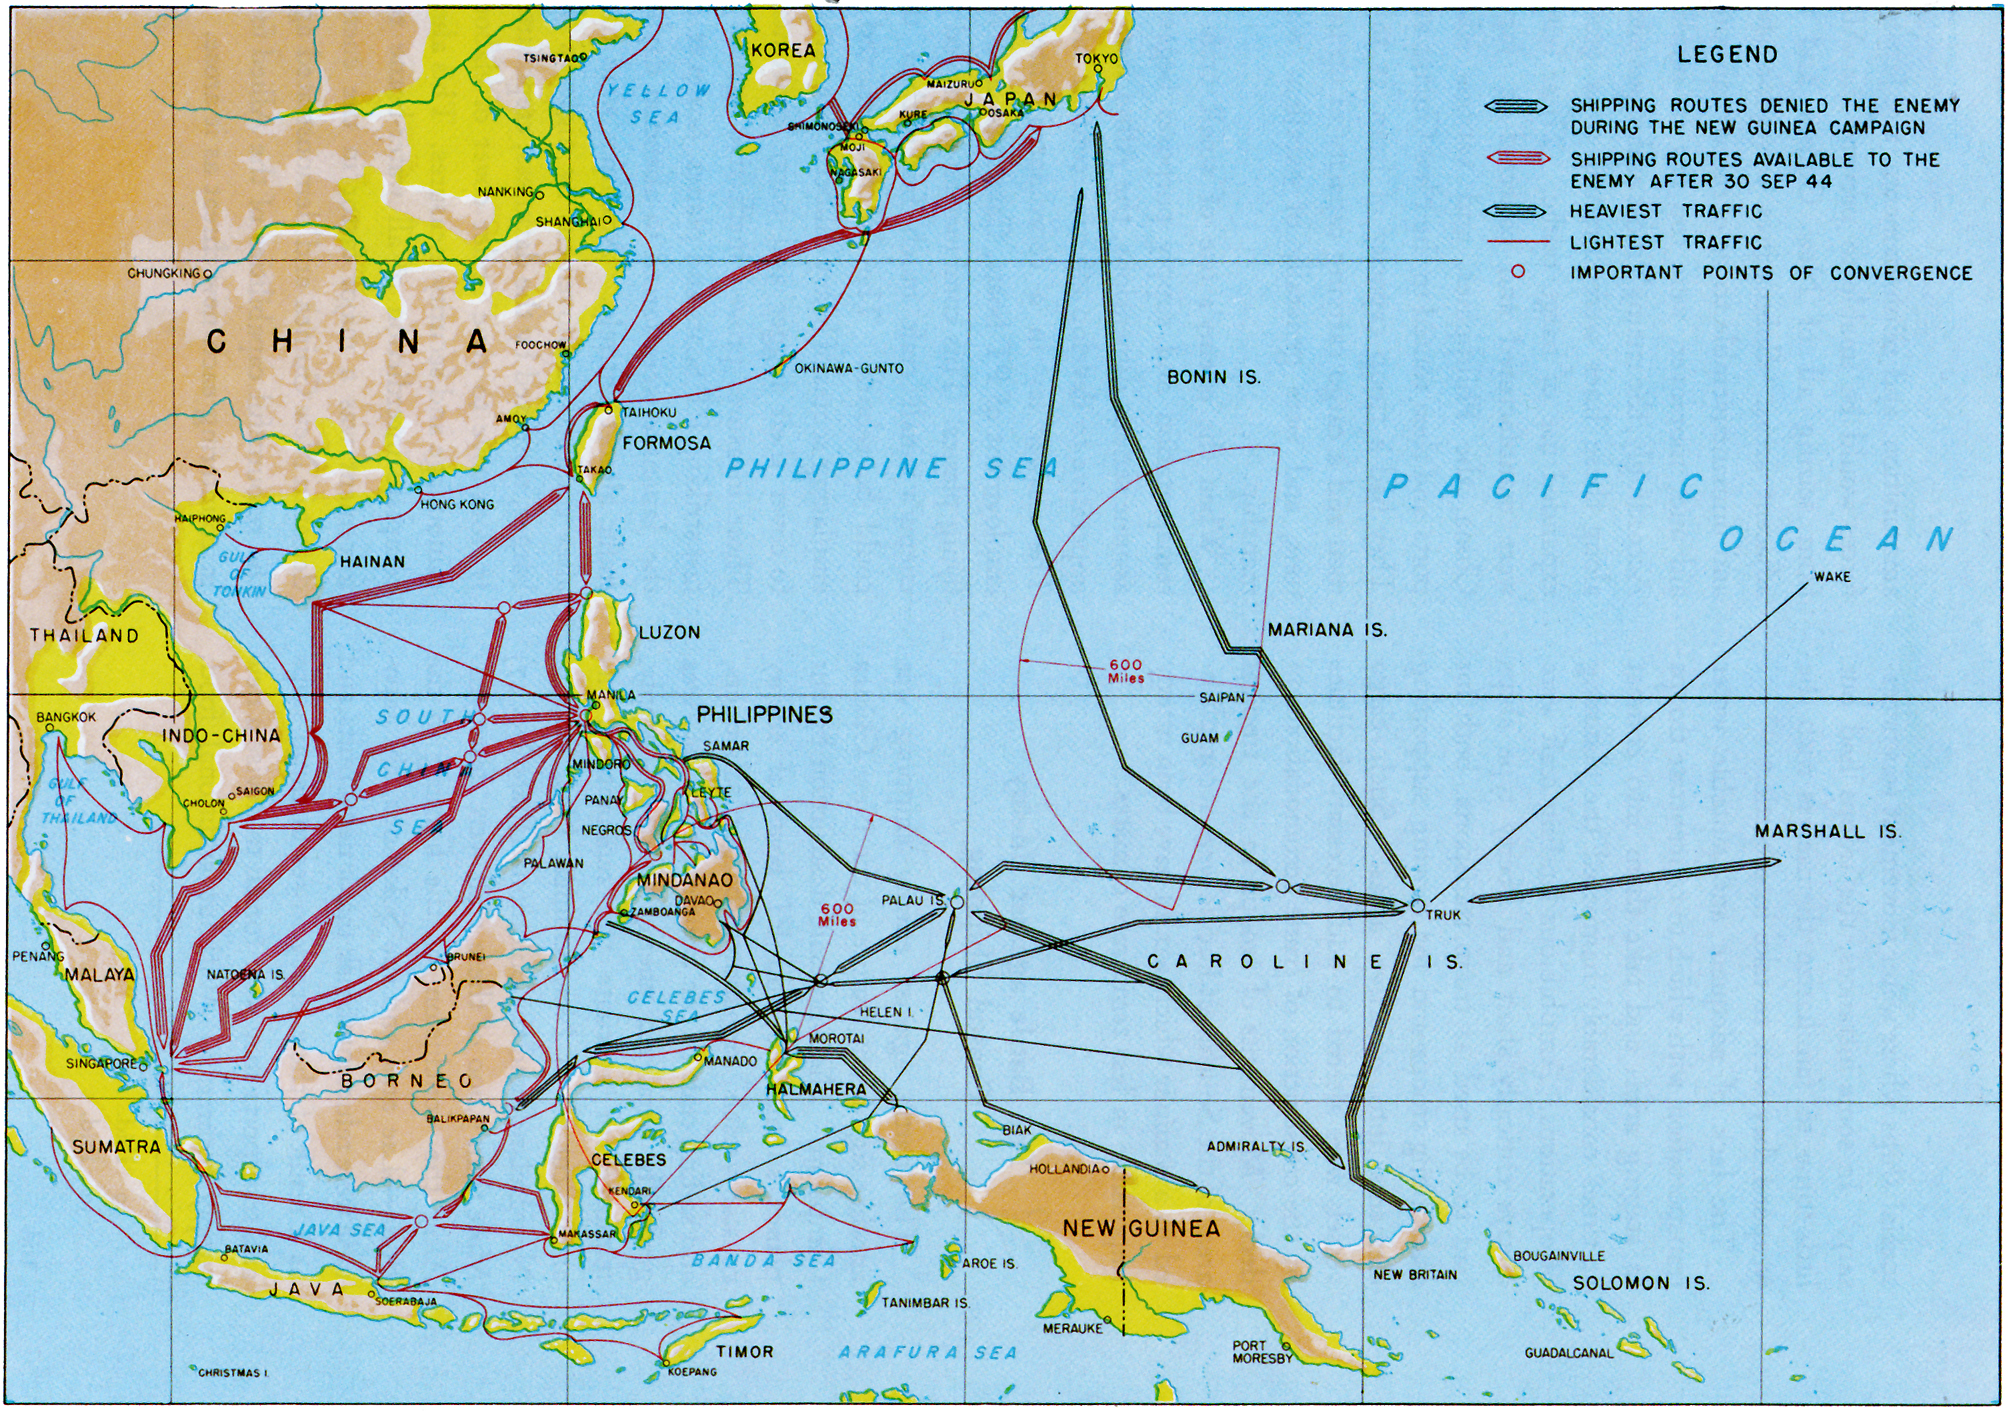
\includegraphics[angle=270]{cmap}

\section{Recognition Manual (Short, Metric)}
\centering
\begin{tabularx}{\textwidth}{|r|l|l|l|l|X|}
\hline
\textbf{Name} & \textbf{Speed (kn)} & \textbf{Length (m)} & \textbf{Mast (m)} & \textbf{Draft (m)} & \textbf{Aspect}\\
\hline
 Auxilary Subchaser & $17.00$ & $63.00$ & $11.40$ & $4.20$ & $5.5263$ \\
\hline
Agano Light Cruiser & $35.00$ & $175.00$ & $23.60$ & $5.70$ & $7.4153$ \\
\hline
Akikaze Destroyer & $34.00$ & $102.50$ & $21.80$ & $2.90$ & $4.7018$ \\
\hline
Akita Maru & $13.50$ & $105.00$ & $16.00$ & $7.30$ & $6.5625$ \\
\hline
Akitsu Escort Carrier & $20.00$ & $143.75$ & $35.70$ & $7.84$ & $4.0266$ \\
\hline
Akizuki Destroyer & $33.00$ & $135.00$ & $22.80$ & $3.80$ & $5.9211$ \\
\hline
Armed Merchant Cruiser & $17.50$ & $155.00$ & $26.80$ & $8.70$ & $5.7836$ \\
\hline
Armed Trawler & $12.00$ & $62.00$ & $13.50$ & $4.20$ & $4.5926$ \\
\hline
Asashio Destroyer & $35.00$ & $118.00$ & $27.00$ & $3.40$ & $4.3704$ \\
\hline
Atami Gunboat & $20.00$ & $45.00$ & $7.80$ & $1.10$ & $5.7692$ \\
\hline
Attacker Escort Carrier & $18.00$ & $152.00$ & $33.80$ & $8.20$ & $4.4970$ \\
\hline
Baltimore Heavy Cruiser & $33.00$ & $205.00$ & $30.60$ & $6.50$ & $6.6993$ \\
\hline
Biyo Maru & $12.00$ & $120.00$ & $20.10$ & $7.50$ & $5.9701$ \\
\hline
Black Swan Sloop & $19.50$ & $91.30$ & $27.20$ & $3.50$ & $3.3566$ \\
\hline
Bogue Escort Carrier & $18.00$ & $152.00$ & $11.30$ & $8.20$ & $13.4513$ \\
\hline
British Medium Old Tanker & $10.00$ & $91.50$ & $11.00$ & $4.50$ & $8.3182$ \\
\hline
Brooklyn Light Cruiser & $32.50$ & $185.00$ & $32.30$ & $7.00$ & $5.7276$ \\
\hline
Buckley Destroyer Escort & $24.00$ & $93.20$ & $21.10$ & $3.40$ & $4.4171$ \\
\hline
Buzyun Maru & $11.00$ & $103.00$ & $9.80$ & $6.40$ & $10.5102$ \\
\hline
Casablanca Escort Carrier & $19.00$ & $156.00$ & $13.90$ & $6.30$ & $11.2230$ \\
\hline
Chitose Seaplane Tender & $28.90$ & $192.50$ & $32.60$ & $7.50$ & $5.9049$ \\
\hline
Clemson Destroyer & $35.00$ & $95.00$ & $28.80$ & $3.10$ & $3.2986$ \\
\hline
Cleveland Light Cruiser & $32.50$ & $185.00$ & $36.20$ & $6.60$ & $5.1105$ \\
\hline
Coastal Composite Freighter & $13.00$ & $80.77$ & $17.90$ & $5.48$ & $4.5123$ \\
\hline
Colorado Battleship & $21.00$ & $190.20$ & $43.90$ & $9.10$ & $4.3326$ \\
\hline
Conte Verde Liner & $21.00$ & $173.74$ & $28.60$ & $7.50$ & $6.0748$ \\
\hline
Dido Light Cruiser & $32.00$ & $156.00$ & $36.50$ & $6.30$ & $4.2740$ \\
\hline
Elco Torpedo Boat & $44.00$ & $24.70$ & $5.30$ & $1.20$ & $4.6604$ \\
\hline
Elite Black Swan Sloop & $19.50$ & $91.30$ & $27.20$ & $3.50$ & $3.3566$ \\
\hline
Etorofu Escort & $19.70$ & $66.00$ & $17.90$ & $2.93$ & $3.6872$ \\
\hline
Evarts Destroyer Escort & $19.00$ & $89.50$ & $27.70$ & $3.40$ & $3.2310$ \\
\hline
Fiji Light Cruiser & $32.00$ & $169.00$ & $43.90$ & $5.00$ & $3.8497$ \\
\hline
Fishing boat & $10.00$ & $38.00$ & $18.70$ & $1.80$ & $2.0321$ \\
\hline
Fishing boat & $10.00$ & $38.00$ & $18.70$ & $1.80$ & $2.0321$ \\
\hline
Fishing Boat & $8.00$ & $34.00$ & $7.90$ & $2.40$ & $4.3038$ \\
\hline
Fishing Trawler & $12.00$ & $62.00$ & $13.50$ & $4.20$ & $4.5926$ \\
\hline
Fleet Carrier & $32.50$ & $250.00$ & $54.40$ & $6.80$ & $4.5956$ \\
\hline
Fletcher Destroyer & $35.00$ & $115.00$ & $28.00$ & $4.90$ & $4.1071$ \\
\hline
Flower Corvette & $16.00$ & $60.60$ & $19.70$ & $3.50$ & $3.0761$ \\
\hline
Fubuki Destroyer & $38.00$ & $118.50$ & $22.60$ & $3.50$ & $5.2434$ \\
\hline
Furutaka Heavy Cruiser & $33.00$ & $188.00$ & $25.90$ & $5.20$ & $7.2587$ \\
\hline
Fuso Battleship & $24.70$ & $212.00$ & $48.30$ & $9.50$ & $4.3892$ \\
\hline
Hakusika Maru & $12.00$ & $135.00$ & $20.30$ & $8.70$ & $6.6502$ \\
\hline
Haruna Maru & $11.00$ & $76.00$ & $19.70$ & $4.60$ & $3.8579$ \\
\hline
Heito Maru & $17.00$ & $103.60$ & $16.60$ & $6.50$ & $6.2410$ \\
\hline
Hira Gunboat & $20.00$ & $55.00$ & $10.10$ & $1.10$ & $5.4455$ \\
\hline
Hiryu Fleet Carrier & $34.30$ & $223.30$ & $37.20$ & $7.50$ & $6.0027$ \\
\hline
Horai Maru & $17.00$ & $137.46$ & $25.60$ & $8.53$ & $5.3695$ \\
\hline
Iowa Battleship & $33.00$ & $270.40$ & $44.30$ & $11.00$ & $6.1038$ \\
\hline
Ise Battleship & $25.60$ & $220.00$ & $44.50$ & $9.50$ & $4.9438$ \\
\hline
Ise Battleship (Late War) & $25.60$ & $220.00$ & $49.20$ & $9.50$ & $4.4715$ \\
\hline
J Class Destroyer & $36.00$ & $108.50$ & $28.00$ & $4.60$ & $3.8750$ \\
\hline
JC Butler Destroyer Escort & $24.00$ & $93.30$ & $28.10$ & $2.80$ & $3.3203$ \\
\hline
Junk & $10.00$ & $19.60$ & $17.70$ & $1.20$ & $1.1073$ \\
\hline
Kasagisan Maru & $12.50$ & $86.80$ & $18.10$ & $6.10$ & $4.7956$ \\
\hline
\end{tabularx}
\pagebreak

\begin{tabularx}{\textwidth}{|r|l|l|l|l|X|}
\hline
\textbf{Name} & \textbf{Speed (kn)} & \textbf{Length (m)} & \textbf{Mast (m)} & \textbf{Draft (m)} & \textbf{Aspect}\\
\hline
Kent Heavy Cruiser & $31.50$ & $183.00$ & $21.80$ & $5.00$ & $8.3945$ \\
\hline
King George V Battleship & $27.00$ & $244.00$ & $53.90$ & $9.10$ & $4.5269$ \\
\hline
Kinposan Maru & $14.50$ & $108.00$ & $18.50$ & $6.60$ & $5.8378$ \\
\hline
Kisaragi Destroyer & $37.00$ & $102.00$ & $11.20$ & $3.00$ & $9.1071$ \\
\hline
Kiturin Maru & $18.50$ & $130.00$ & $25.70$ & $8.60$ & $5.0584$ \\
\hline
Kongo Battleship & $30.50$ & $220.00$ & $42.50$ & $8.50$ & $5.1765$ \\
\hline
Kuma Light Cruiser & $36.00$ & $163.00$ & $35.60$ & $6.10$ & $4.5787$ \\
\hline
Landing Ship Tank & $10.80$ & $98.70$ & $25.20$ & $3.30$ & $3.9167$ \\
\hline
Large German Tanker & $18.00$ & $190.00$ & $24.20$ & $10.70$ & $7.8512$ \\
\hline
Large Sampan & $10.00$ & $35.00$ & $26.90$ & $2.20$ & $1.3011$ \\
\hline
Liberty Cargo & $13.00$ & $147.00$ & $21.00$ & $5.80$ & $7.0000$ \\
\hline
Maya Heavy Cruiser & $34.00$ & $204.00$ & $33.50$ & $5.90$ & $6.0896$ \\
\hline
Medium Modern Passenger/Freighter & $16.00$ & $105.00$ & $27.40$ & $7.30$ & $3.8321$ \\
\hline
Minekaze Destroyer & $39.00$ & $102.60$ & $21.80$ & $2.90$ & $4.7064$ \\
\hline
Mogami Heavy Cruiser & $35.00$ & $200.00$ & $35.00$ & $6.70$ & $5.7143$ \\
\hline
Momi Destroyer & $18.00$ & $102.60$ & $11.10$ & $2.93$ & $9.2432$ \\
\hline
Momoyama Maru & $11.00$ & $120.00$ & $16.00$ & $4.70$ & $7.5000$ \\
\hline
Momoyama Maru & $11.00$ & $120.00$ & $16.00$ & $4.70$ & $7.5000$ \\
\hline
Mutsuki Destroyer & $37.00$ & $102.00$ & $11.20$ & $3.00$ & $9.1071$ \\
\hline
Nagara Maru & $19.00$ & $137.00$ & $20.50$ & $7.50$ & $6.6829$ \\
\hline
Naka Light Cruiser & $35.25$ & $162.00$ & $31.30$ & $5.10$ & $5.1757$ \\
\hline
Nevada Battleship & $20.50$ & $190.20$ & $43.90$ & $9.10$ & $4.3326$ \\
\hline
New Mexico Battleship & $22.00$ & $190.00$ & $42.00$ & $10.00$ & $4.5238$ \\
\hline
Nippon Maru & $20.00$ & $150.00$ & $16.70$ & $8.60$ & $8.9820$ \\
\hline
North Carolina Battleship & $27.00$ & $220.00$ & $33.40$ & $9.00$ & $6.5868$ \\
\hline
Northampton Heavy Cruiser & $32.70$ & $183.00$ & $49.00$ & $7.00$ & $3.7347$ \\
\hline
Okinoshima Minelayer & $20.00$ & $123.40$ & $28.50$ & $4.80$ & $4.3298$ \\
\hline
Old Raked Bow Split Merchant & $11.00$ & $120.00$ & $17.30$ & $4.70$ & $6.9364$ \\
\hline
Omaha Light Cruiser & $35.00$ & $168.00$ & $19.50$ & $4.50$ & $8.6154$ \\
\hline
Patrol Boat 102 & $35.00$ & $95.00$ & $28.70$ & $3.10$ & $3.3101$ \\
\hline
Pennsylvania Battleship & $21.00$ & $190.20$ & $43.90$ & $9.10$ & $4.3326$ \\
\hline
Pocket Battleship & $28.50$ & $183.00$ & $37.90$ & $7.00$ & $4.8285$ \\
\hline
River class Frigate & $20.00$ & $91.50$ & $25.90$ & $4.00$ & $3.5328$ \\
\hline
Sampan & $10.00$ & $19.50$ & $16.50$ & $1.20$ & $1.1818$ \\
\hline
Schnellboat & $44.00$ & $24.70$ & $5.30$ & $1.20$ & $4.6604$ \\
\hline
Shimushu Escort & $20.00$ & $70.00$ & $24.50$ & $2.93$ & $2.8571$ \\
\hline
Shiratsuyu Destroyer & $34.00$ & $108.00$ & $22.00$ & $3.00$ & $4.9091$ \\
\hline
Shokaku Fleet Carrier & $34.50$ & $250.00$ & $32.40$ & $8.70$ & $7.7160$ \\
\hline
Small Old Split Freighter & $17.00$ & $80.50$ & $17.90$ & $3.70$ & $4.4972$ \\
\hline
Small Split Freighter & $12.50$ & $86.87$ & $18.10$ & $6.10$ & $4.7994$ \\
\hline
Somers Destroyer & $37.00$ & $116.00$ & $31.50$ & $4.20$ & $3.6825$ \\
\hline
Submarine Tender & $18.00$ & $201.00$ & $22.40$ & $9.40$ & $8.9732$ \\
\hline
T3 Tanker & $18.00$ & $190.00$ & $25.50$ & $10.70$ & $7.4510$ \\
\hline
Taiho Fleet Carrier & $33.30$ & $253.70$ & $46.20$ & $9.50$ & $5.4913$ \\
\hline
Taihosan Maru & $13.00$ & $80.50$ & $17.90$ & $3.70$ & $4.4972$ \\
\hline
Taiyo Escort Carrier & $21.00$ & $180.10$ & $15.10$ & $7.50$ & $11.9272$ \\
\hline
Takao Heavy Cruiser & $36.50$ & $204.00$ & $35.30$ & $6.00$ & $5.7790$ \\
\hline
Tennessee Battleship & $20.50$ & $190.00$ & $42.00$ & $10.00$ & $4.5238$ \\
\hline
Tennessee Battleship & $20.50$ & $190.20$ & $43.90$ & $9.10$ & $4.3326$ \\
\hline
Tribal Destroyer & $36.50$ & $115.00$ & $15.40$ & $4.00$ & $7.4675$ \\
\hline
Troop Transport & $16.00$ & $152.00$ & $23.20$ & $8.50$ & $6.5517$ \\
\hline
Tug Boat & $15.00$ & $63.00$ & $11.50$ & $4.20$ & $5.4783$ \\
\hline
Tyohei Maru & $13.00$ & $79.00$ & $14.30$ & $4.60$ & $5.5245$ \\
\hline
Type C Escort & $19.00$ & $89.50$ & $27.70$ & $3.40$ & $3.2310$ \\
\hline
Type D Escort & $19.00$ & $89.50$ & $27.70$ & $3.40$ & $3.2310$ \\
\hline
\end{tabularx}
\pagebreak

\begin{tabularx}{\textwidth}{|r|l|l|l|l|X|}
\hline
\textbf{Name} & \textbf{Speed (kn)} & \textbf{Length (m)} & \textbf{Mast (m)} & \textbf{Draft (m)} & \textbf{Aspect}\\
\hline
V.W Destroyer & $34.00$ & $95.00$ & $21.00$ & $3.20$ & $4.5238$ \\
\hline
Victory Cargo & $17.00$ & $139.60$ & $21.80$ & $7.30$ & $6.4037$ \\
\hline
Wakatake Patrol Boat & $18.00$ & $102.60$ & $21.70$ & $2.93$ & $4.7281$ \\
\hline
West Virginia Battleship & $21.00$ & $190.00$ & $42.00$ & $10.00$ & $4.5238$ \\
\hline
Yamato Battleship & $27.40$ & $263.00$ & $39.20$ & $10.80$ & $6.7092$ \\
\hline
Yugumo Destroyer & $35.00$ & $118.00$ & $11.50$ & $3.40$ & $10.2609$ \\
\hline
Z Class Destroyer & $38.00$ & $118.50$ & $22.60$ & $3.50$ & $5.2434$ \\
\hline
Zinbu Maru & $10.00$ & $120.00$ & $18.60$ & $4.70$ & $6.4516$ \\
\hline
\end{tabularx}
\pagebreak



%%%END END END
\pagebreak
\begin{thebibliography}{9}

\bibitem{angrHandB}
  Karl Hahl,
  Kriegsmarine Angriffscheibe Handbuch,
  p. 15,
  2008.
  
\bibitem{tvreAcqData}
http://www.tvre.org/en/acquiring-torpedo-firing-data,
Acquiring torpedo firing data,
2015.

\bibitem{okane90Angles}
Corey "Gutted" Hardwell,
Silent Hunter IV 90\degree - AOB Firing Angles,
circ. 2008(?).

\bibitem{subsim}
http://www.subsim.com

\bibitem{arcSin}
MathOnWeb,
%http://mathonweb.com/help_ebook/html/functions_2.htm,
The arcsin function,
Accessed 17.08.2015,


\end{thebibliography}




\end{document}

